
\begin{frame}
\frametitle{Fechas importantes de entrega de proyectos (1)}

\begin{itemize}
\item Fecha de asignación: fecha en que se da a conocer al grupo el trabajo a elaborar
\item Fecha de entrega sin penalización: 14 dias naturales despues de la fecha de asignación
\item Proyecto entregado despues de ha fecha de penalización se le aplica una penalización de 25 PUNTOS
\item Fecha de cierre: 21 días naturales despues de la fecha de asignación. 
\end{itemize}
\begin{block}{Regla ``CANTU''}
\begin{itemize}
\item Ningún proyecto será revisado despues de la fecha de cierre. Se programarán las entregas para cerrar y no permitir entregas tardías. 
\end{itemize}
\end{block}
\end{frame}

\begin{frame}
\frametitle{Fechas importantes de entrega de proyectos (2)}
\begin{block}{Grafo ``DAFNE''}
\begin{center}
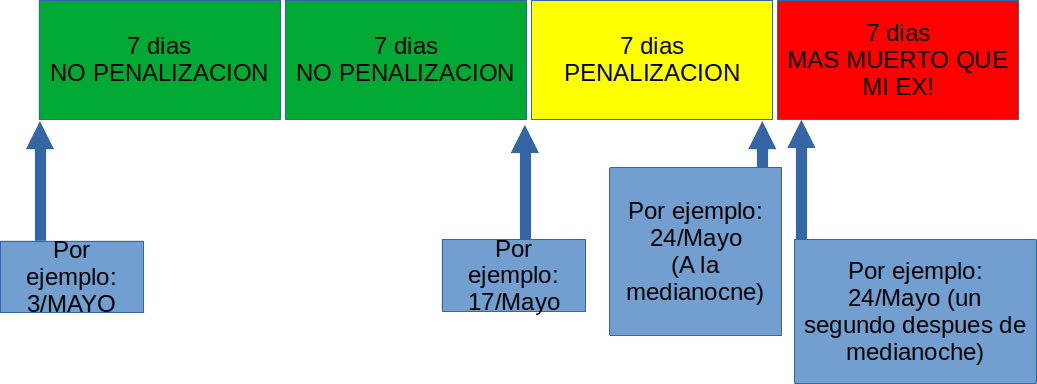
\includegraphics[width=12cm]{FechasEntrega/Grafo_Fechas.png}
\end{center}
\begin{itemize}
\item En el momento de publicar la tarea, se incluirá la fecha para no penalización y fecha de cierre.
\end{itemize}
\end{block}

\end{frame}


\begin{frame}
\frametitle{¿Es posible obtener una calificacion negativa?}
SI
\begin{center}
\begin{tabular}{p{12cm}|c}
\hline
Calificación asignada después de revisión & 70 \\ \hline
(-) Debería entregarse 14/Mayo, lo entregó 21/Mayo (1 minuto antes de la medianoche) & 25 \\
(-) Nombre Archivo MAL & 8 \\ 
(-) Tipo de Archivo MAL & 8 \\ 
(-) Estructura de Directorios INCORRECTA & 8 \\ 
(-) Faltas o Errores en Script  & 8 \\ 
(-) ZIPs dentro del ZIP  & 8 \\ 
(-) Incluir ejecutables (aplica solo cuando el lenguaje es C++)  & 8 \\ \hline
(-) Penalización por Fragmentación de Equipo  & 25 \\ \hline
\textbf{Calificación Final}  & \textbf{-28} \\ \hline
\hline
\hline
\end{tabular}


\end{center}


\end{frame}




